\documentclass[border=5mm]{standalone}
\usepackage{tikz}
\usetikzlibrary{calc, intersections}

\begin{document}
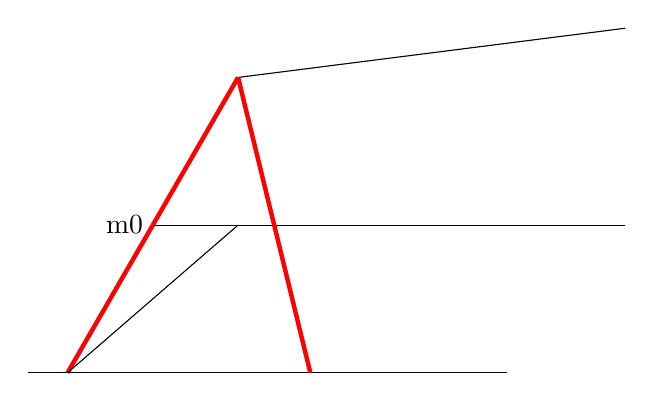
\begin{tikzpicture}


\coordinate[label=left:m0] (m0) at (0,0);
\coordinate (m1) at (1.0825, 1.875);
\coordinate (m2) at (6, 2.5);
\coordinate (m3) at (6,0);
\coordinate (m4) at (1.0825, 0);
\coordinate (m5) at (-1.0825,-1.875);

% nose angle
  \draw[ultra thick,red] (m0) -- (m1);
  \draw[ultra thick,red](m0) -- (m5);

% ms bottom
  \draw (m0) -- (m3);

% bearing brace
\draw (m4) -- (m5);

% ms front taper
  \draw (m1) -- (m2);

% prop shaft line

  \draw ($ (m5) + (-0.5,0) $) -- (4.5, -1.875);

  \draw[ultra thick,red] (m1) -- (2, -1.875);


\end{tikzpicture}
\end{document}

